\begin{frame}{\textsc{Часть I}}{Буря 25-26 августа 2018 года}
\begin{figure}
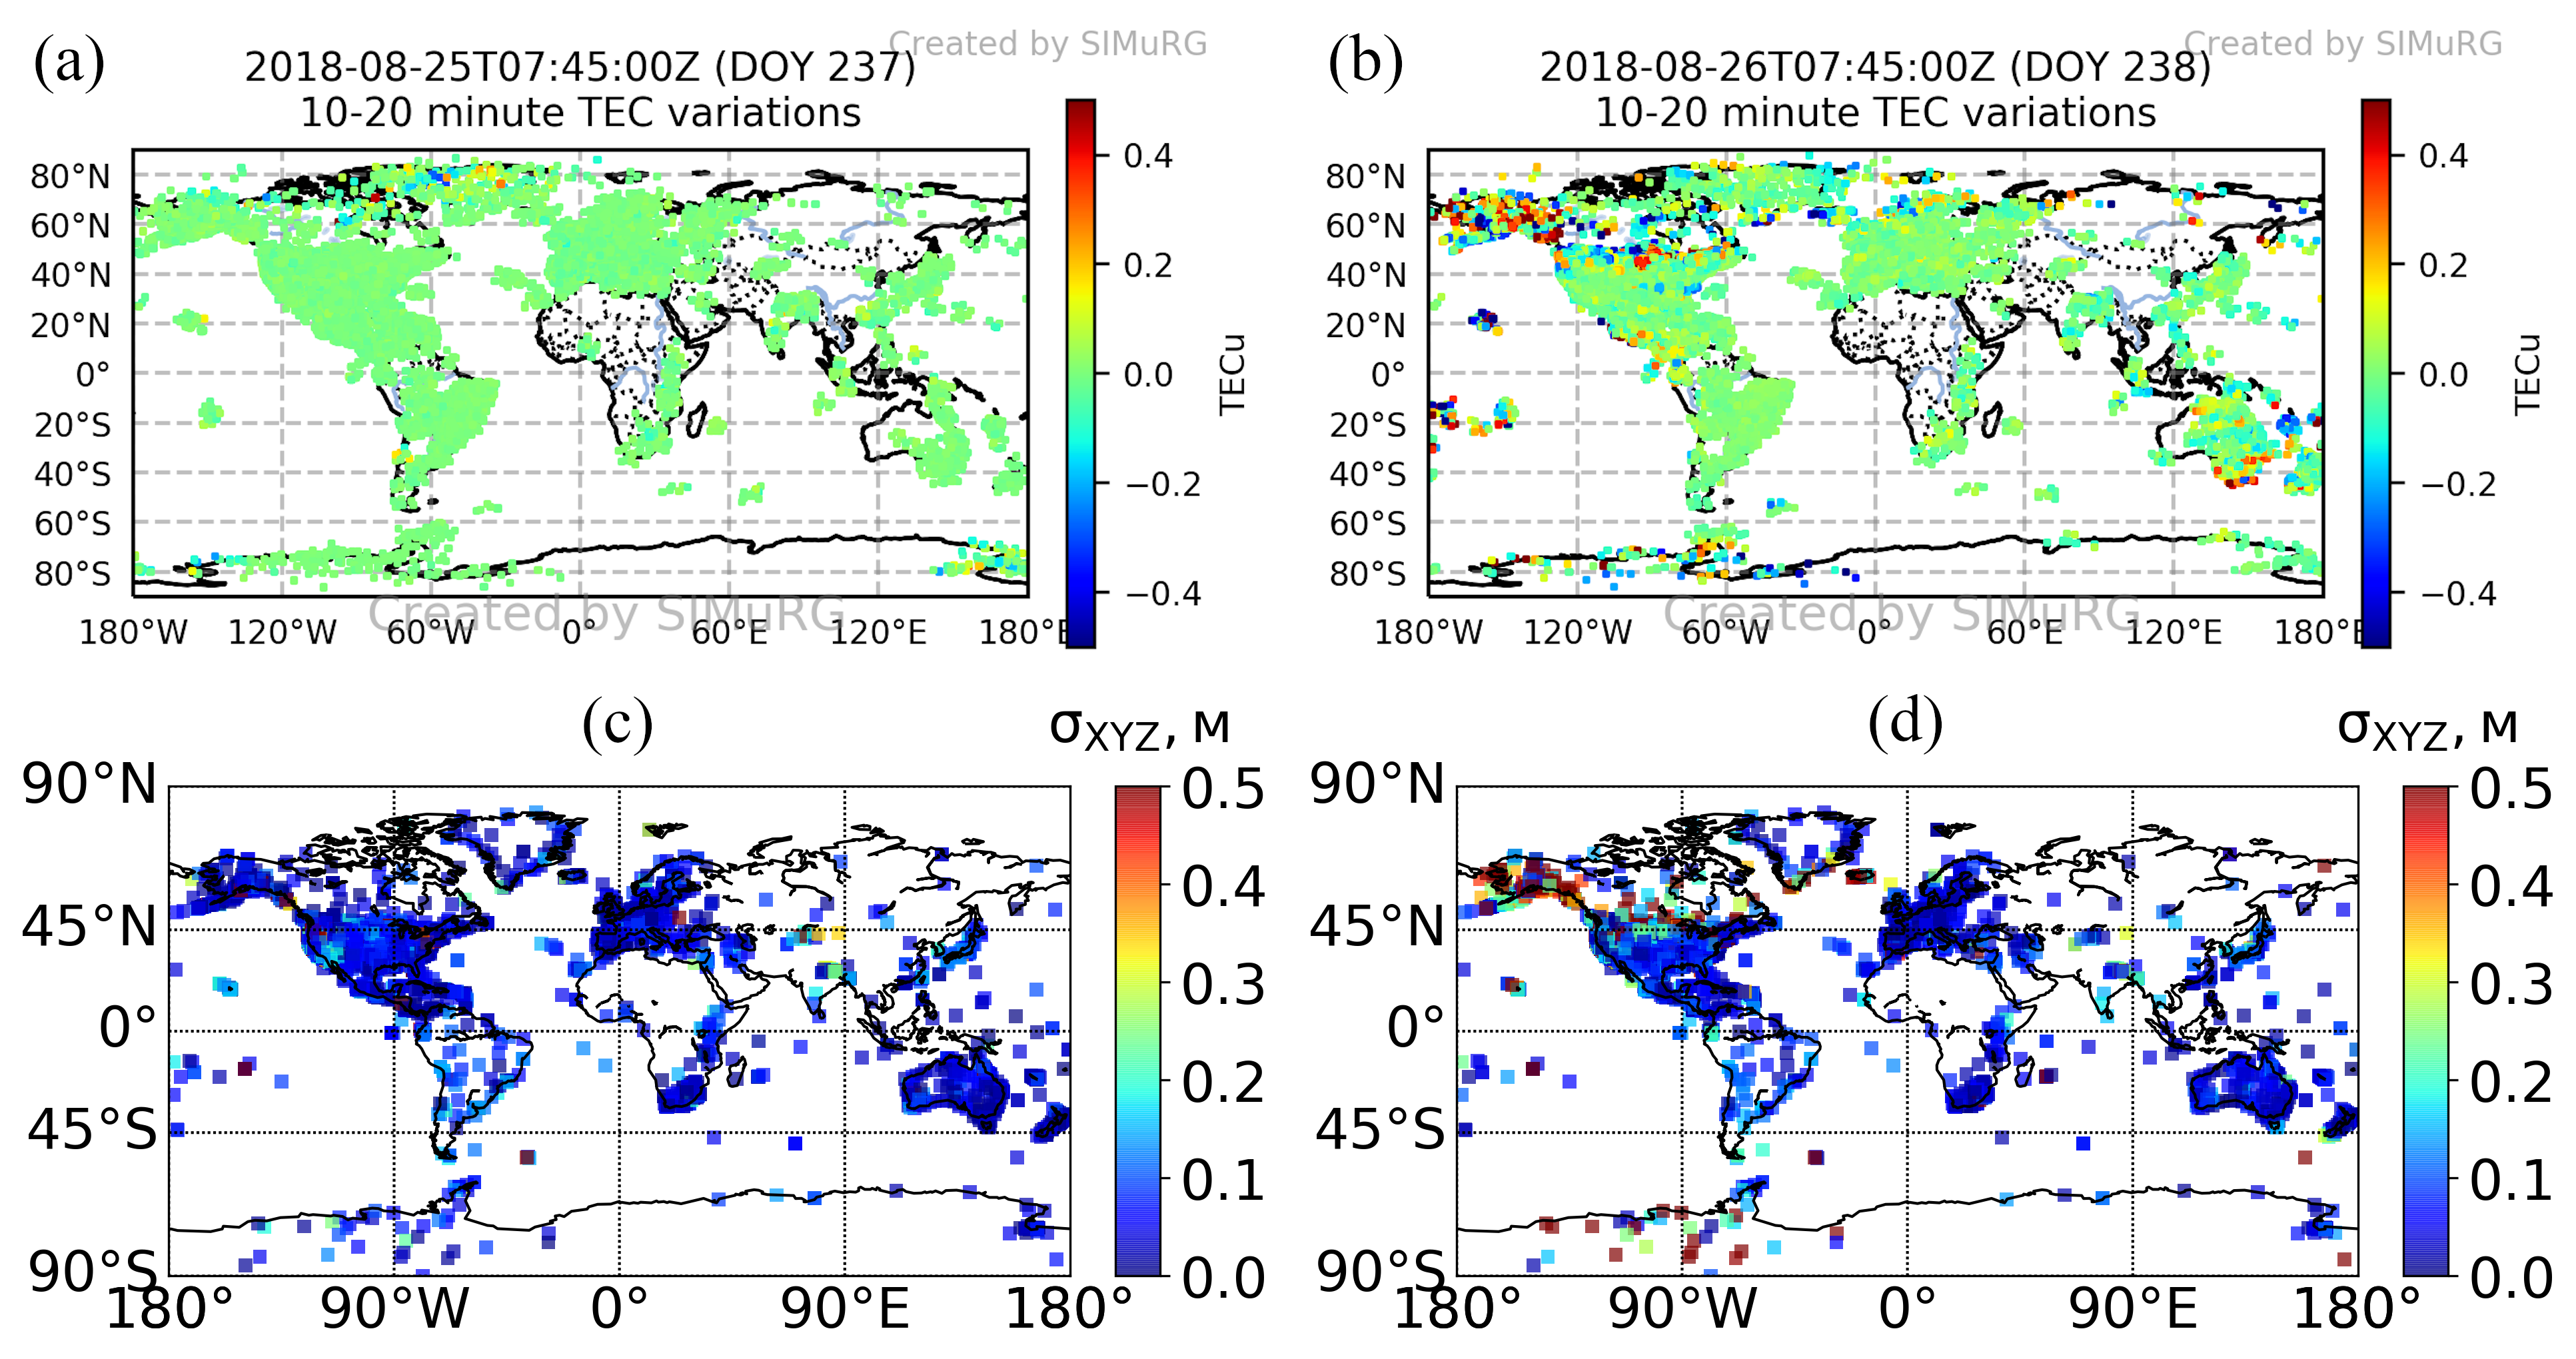
\includegraphics[width=\textwidth]{../fig/2018-237-238-07-45.png}    
\end{figure} 
\end{frame}

\begin{frame}{\textsc{Часть I}}{Буря 25-26 августа 2018 года}
\begin{figure}
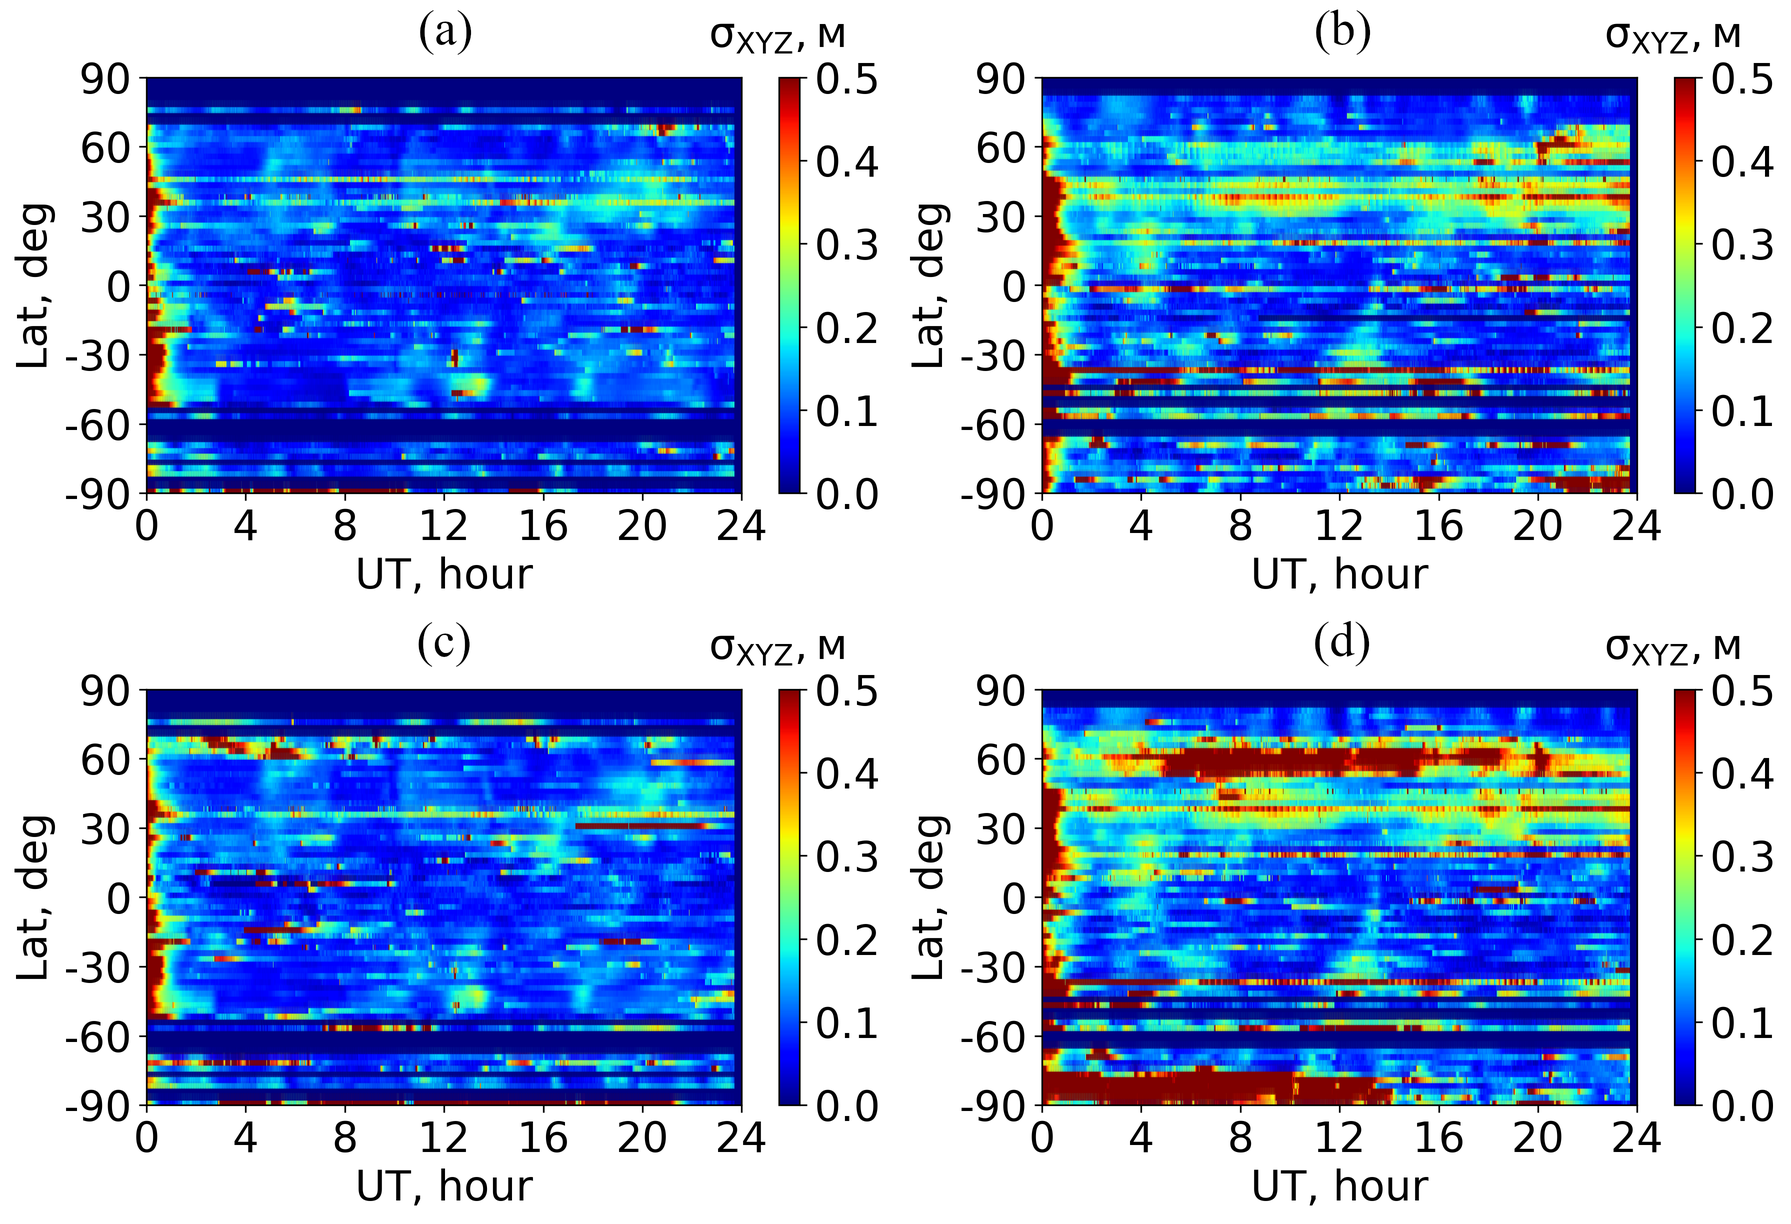
\includegraphics[width=0.77\textwidth]{../fig/2018-237-238.png}   
\end{figure} 
\end{frame}

\begin{frame}{\textsc{Часть I}}{Буря 21-22 июня 2015 года}
\begin{figure}
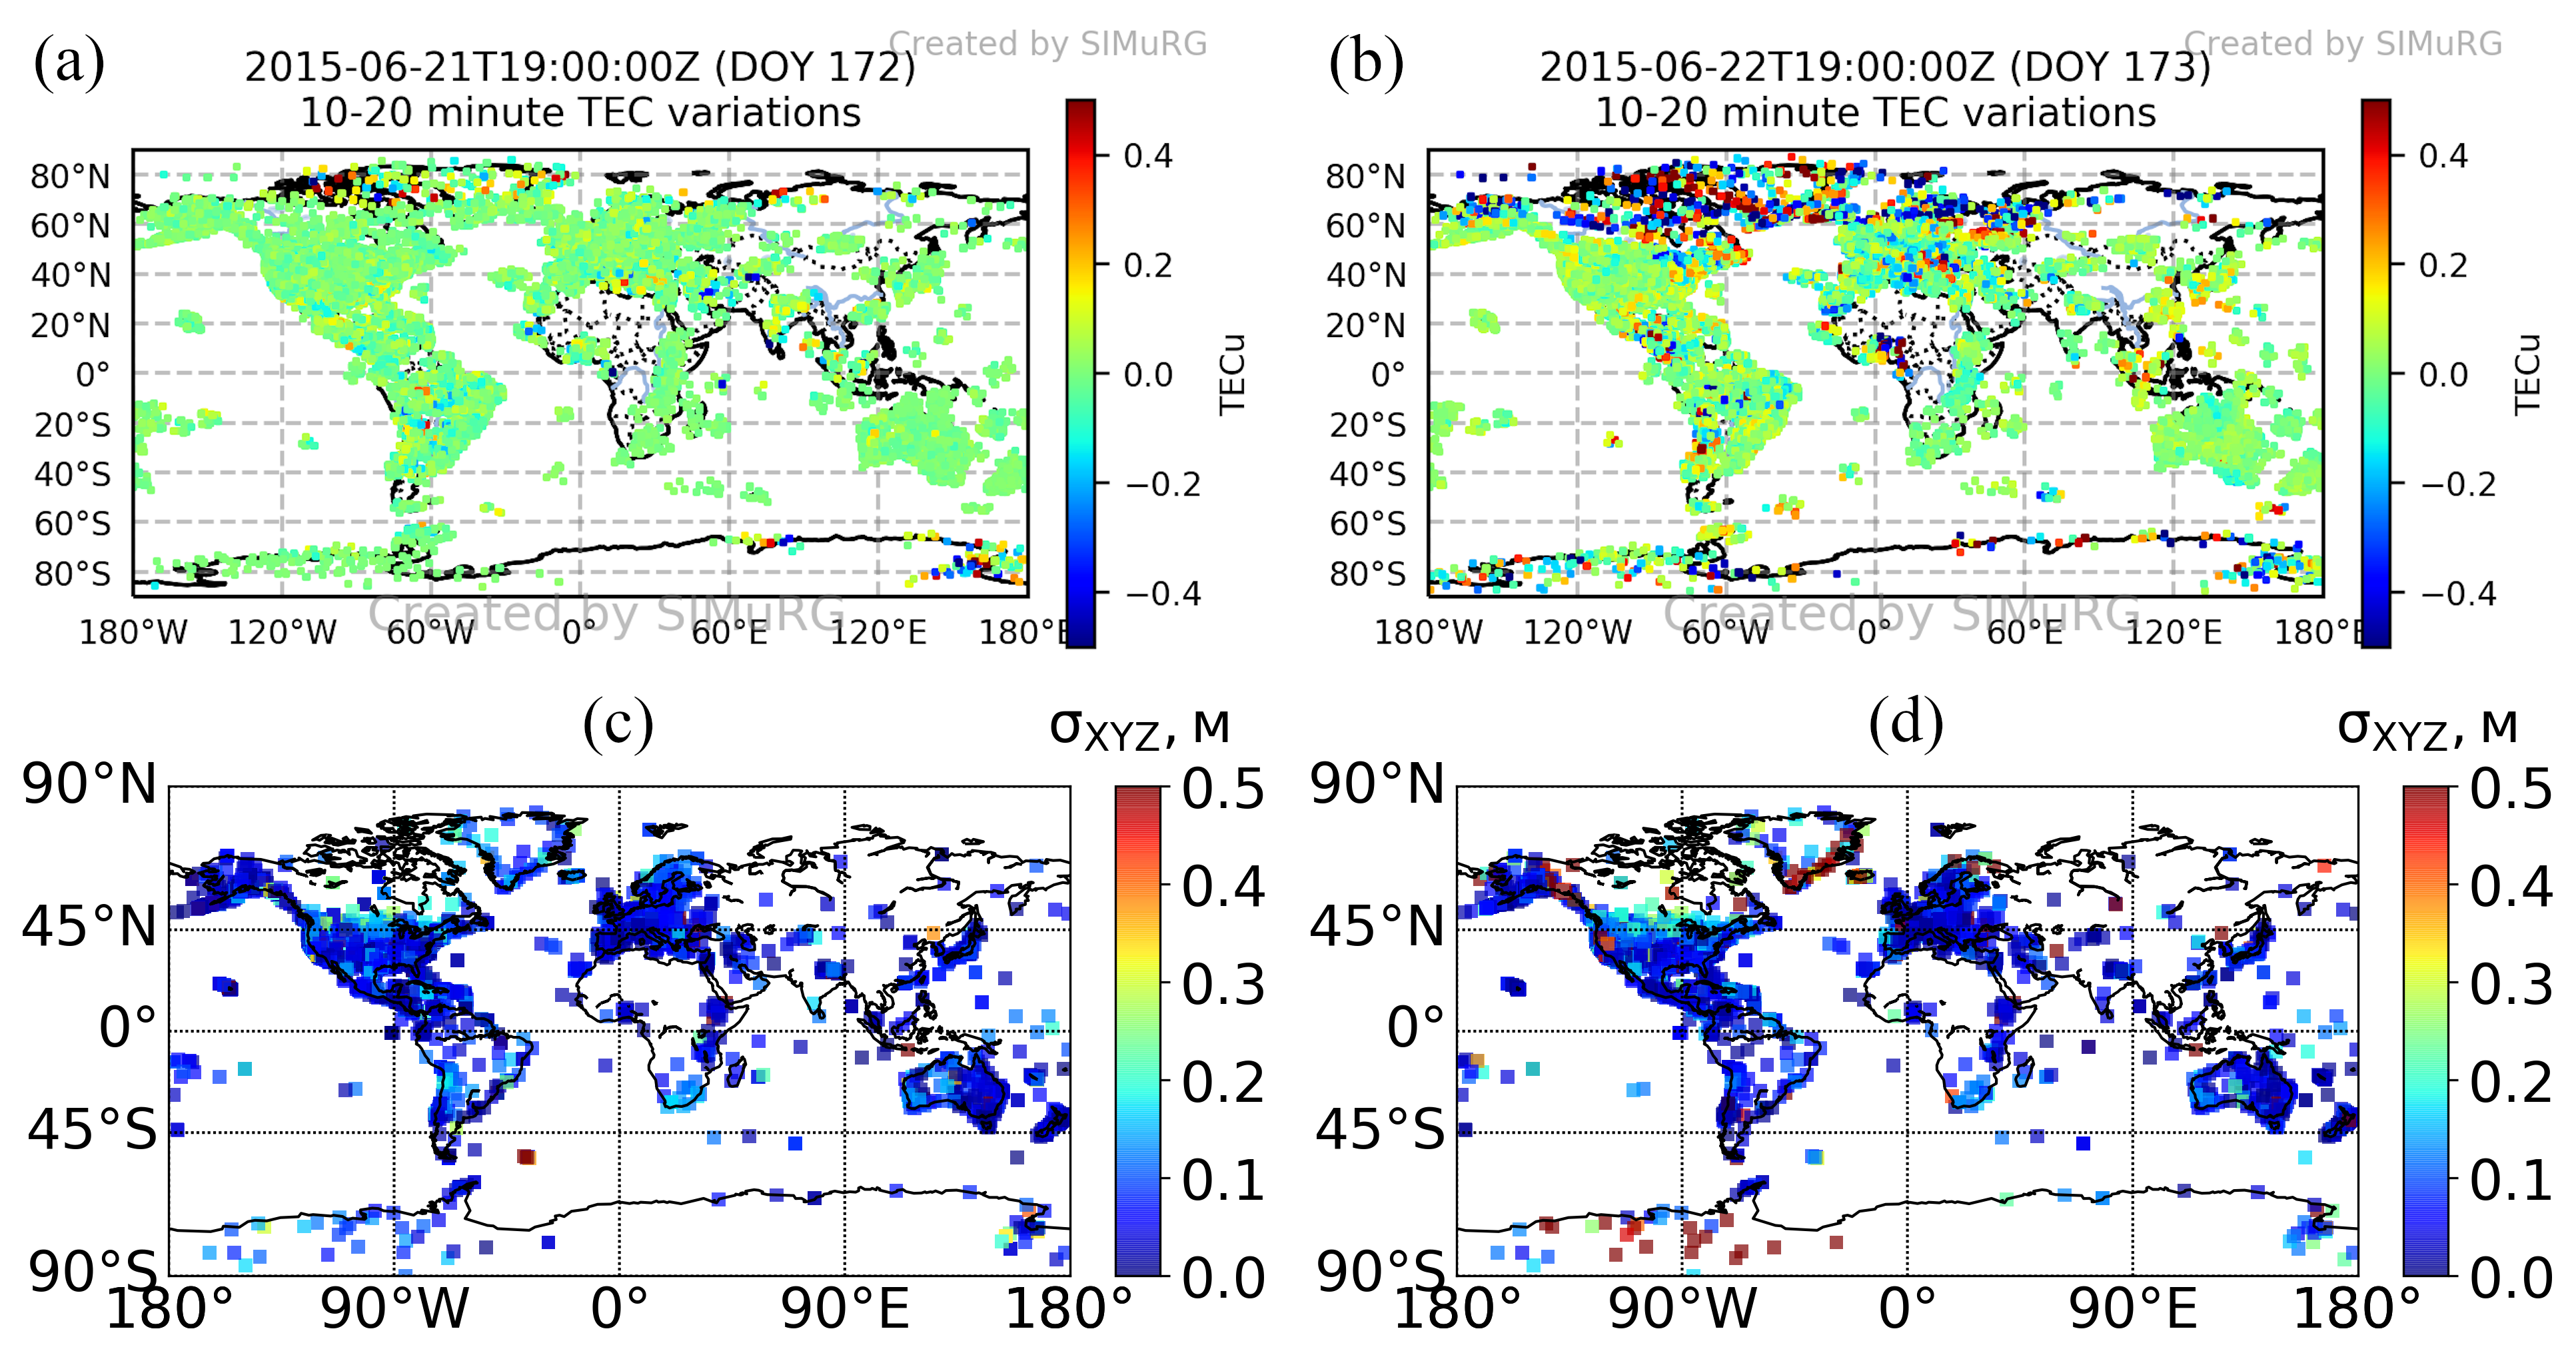
\includegraphics[width=\textwidth]{../fig/2015-172-173-19-00.png}   
\end{figure} 
\end{frame}

\begin{frame}{\textsc{Часть I}}{Буря 21-22 июня 2015 года}
\begin{figure}
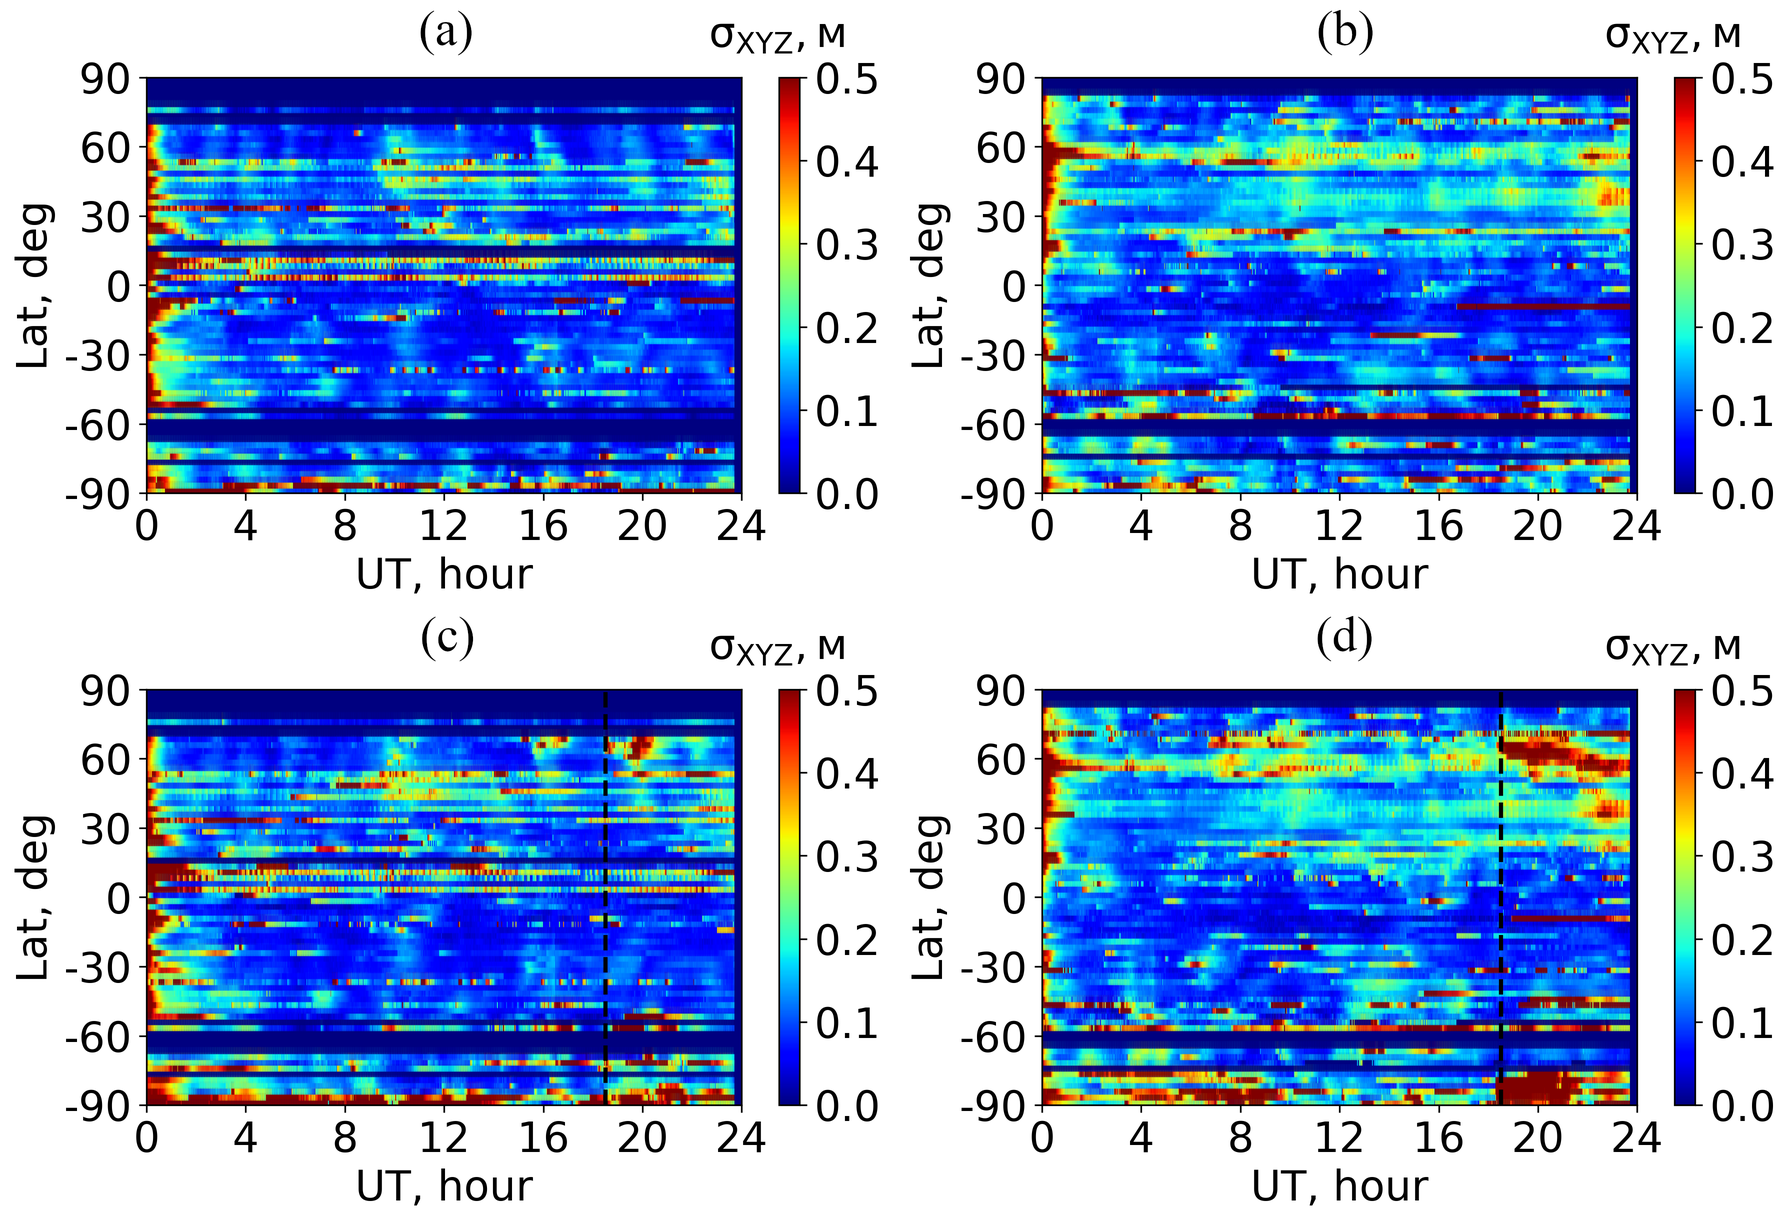
\includegraphics[width=0.77\textwidth]{../fig/2015-172-173.png}   
\end{figure} 
\end{frame}

\begin{frame}{\textsc{Часть I}}{Результаты\footnote[1]{{\tiny Yu. Yasyukevich, R. Vasilyev, K. Ratovsky, A. Setov, M. Globa, \begin{bf}S. Syrovatskii\end{bf}, A. Yasyukevich, A. Kiselev, A. Vesnin. Small-Scale Ionospheric Irregularities of Auroral Origin at Mid-Latitudes during the 22 June 2015 Magnetic Storm and Their Effect on GPS Positioning // \href{http://dx.doi.org/10.3390/rs12101579}{Remote Sensing}. --- 2020. --- Vol. 12, no. 10.}}}
\begin{enumerate}
\justifying
\item Рассмотрены две геомагнитные бури в период 24-го цикла солнечной активности: за 25-26 августа 2018 года и 21-22 июня 2015 года.
\item Установлено, что точность позиционирования PPP на средних и высоких широтах может снижаться в несколько (\textbf{до 5}) раз.
\item Области снижения пространственно коррелируют с областями максимальных вариаций TEC (\textbf{авроральные регионы}). 
\item Зарегистрированные эффекты по величине \textbf{сравнимы} с эффектами от мощной солнечной вспышки класса X9.3 6 сентября 2018 года и по времени \textbf{продолжительнее}, чем эффекты во время более мощной бури в День святого Патрика (17 марта) 2015 года.
\end{enumerate}  
\end{frame}